\section*{Aufgabe 2}

\subsection*{a)}

	\paragraph{Abbildung 2:}
		RBD für die serielle Komposition
		\begin{figure}[h]
			\centering
			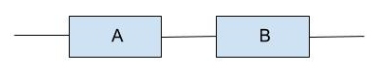
\includegraphics[width=0.5\textwidth]{../2/abbildung_2.png}
		\end{figure}
		\begin{equation*}
			R_2(t) = R_A(t) * R_B(t)
		\end{equation*}
	
	\paragraph{Abbildung 3:}
		RBD für die Systemredundanz
		\begin{figure}[h]
			\centering
			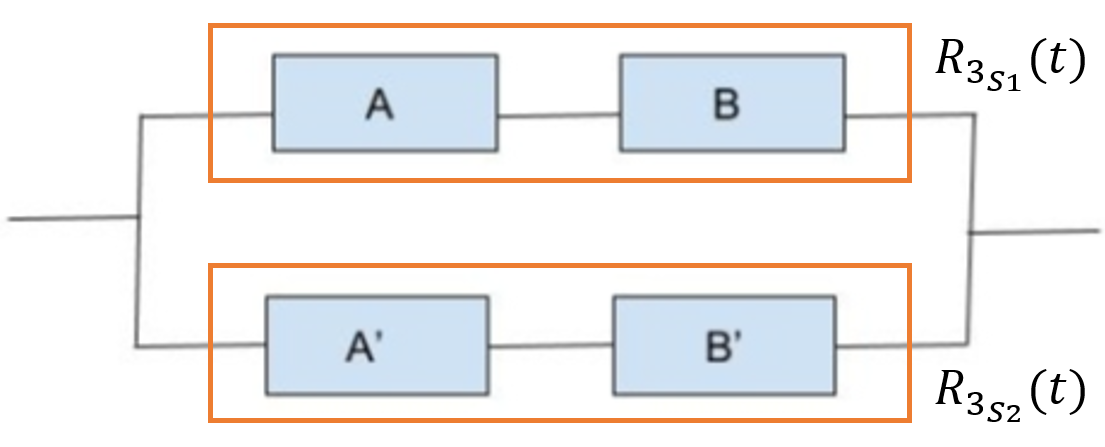
\includegraphics[width=0.5\textwidth]{../2/abbildung_3.png}
		\end{figure}
		\begin{equation*}
			R_{3_{S1}}(t) = R_A(t) * R_B(t)
		\end{equation*}
		\begin{equation*}
			R_{3_{S2}}(t) = R_{A'}(t) * R_{B'}(t)
		\end{equation*}
		\begin{eqnarray*}
			R_3(t) &=&				1 - [ (1 - R_{3_{S1}}(t)) * (1 - R_{3_{S2}}(t)) ]
			\cr &=&					1 - [ (1 - R_A(t) * R_B(t)) * (1 - R_{A'}(t) * R_{B'}(t)) ]
			\cr &\Leftrightarrow&	1 - [ (1 - R_A(t) * R_B(t)) * (1 - R_A(t) * R_B(t)) ]
			\cr &=&					1 - [ (1 - R_A(t) * R_B(t))^2 ]
			\cr &=&					1 - [ 1 - 2*R_A(t)*R_B(t) + R_A(t)^2 * R_B(t)^2 ]
			\cr &=&					R_A(t)^2 * R_B(t)^2 + 2*R_A(t)*R_B(t)
		\end{eqnarray*}
		\begin{eqnarray*}
			R_3(t) &=& R_A(t)^2 * R_B(t)^2 - 2*R_A(t)*R_B(t)
		\end{eqnarray*}
	
	\newpage
	\paragraph{Abbildung 4:}
		RBD für die Komponentenredundanz
		\begin{figure}[h]
			\centering
			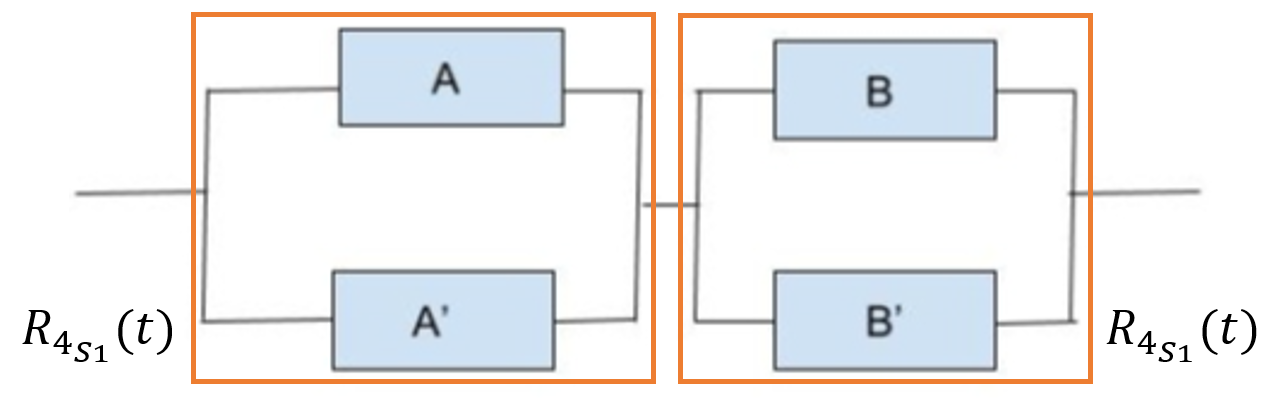
\includegraphics[width=0.5\textwidth]{../2/abbildung_4.png}
		\end{figure}
		\begin{equation*}
			R_{4_{S1}}(t) = 1 - [ (1 - R_A(t)) * (1 - R_{A'}(t)) ]
		\end{equation*}
		\begin{equation*}
			R_{4_{S2}}(t) = 1 - [ (1 - R_B(t)) * (1 - R_{B'}(t)) ]
		\end{equation*}
		\begin{eqnarray*}
			R_4(t) &=&				R_{4_{S1}}(t) * R_{4_{S2}}(t)
			\cr &=&					(1 - [ (1 - R_A(t)) * (1 - R_{A'}(t)) ]) * (1 - [ (1 - R_B(t)) * (1 - R_{B'}(t)) ])
			\cr &\Leftrightarrow&	(1 - [ (1 - R_A(t)) * (1 - R_A(t)) ]) * (1 - [ (1 - R_B(t)) * (1 - R_B(t)) ])
			\cr &=&					(1 - (1 - R_A(t))^2) * (1 - (1 - R_B(t))^2)
			\cr &=&					(1 - (1 - 2*R_A(t) + R_A(t)^2)) * (1 - (1 - 2*R_B(t) + R_B(t)^2))
			\cr &=&					(2*R_A(t) - R_A(t)^2) * (2*R_B(t) - R_B(t)^2)
			%\cr &=&					R_A(t)^2 * R_B(t)^2 + 4*R_A(t)*R_B(t)
			%\cr & &					- 2*R_A(t)^2*R_B(t) - 2*R_A(t)*R_B(t)^2
		\end{eqnarray*}
		\begin{eqnarray*}
			R_4(t) &=& (2*R_A(t) - R_A(t)^2) * (2*R_B(t) - R_B(t)^2)
		\end{eqnarray*}


\subsection*{b)}

	Beispiel:
	\begin{equation*}
		R_A(t) = R_B(t) = 0.5
	\end{equation*}

	\begin{eqnarray*}
		R_2(t)		&=& R_A(t) * R_B(t)
		\cr			&=& 0.5 * 0.5
		\cr			&=& 0.25
		\cr R_3(t)	&=& R_A(t)^2 * R_B(t)^2 - 2*R_A(t)*R_B(t)
		\cr			&=& 0.5^2 * 0.5^2 - 2*0.5*0.5
		\cr			&=& 0.4375
		\cr R_4(t)	&=& (2*R_A(t) - R_A(t)^2) * (2*R_B(t) - R_B(t)^2)
		\cr			&=& (2*0.5 - 0.5^2) * (2*0.5 - 0.5^2)
		\cr			&=& 0.5625
	\end{eqnarray*}
	